\documentclass{article}
\graphicspath{ {./src/} }
\usepackage{../../settings}

\begin{document}
\hexcover{P3 科學筆記本}{學習歷程計畫}{作者:曾嘉禾}{Orchid}{16260621}

\begin{large}
\begin{boxpar}{Orchid}{學習歷程檔案簡述}
    此次實驗討論了實驗環境與反應速率的關係,根據不同的環境討論對於反應速率的影響。在此實驗中我主要擔任上台報告者,為此也常常跟組員討論實驗內容。最後雖然因為時間的關係無法完成海報,但我也因此實驗獲益良多。
\end{boxpar}
\begin{boxpar}{Orchid}{動機}
    在高二的反應速率中,化學老師提到了不同實驗環境對於反應速率的影響。例如溫度與酸鹼值都是引想反應速率的因素。
    經過詢問化學老師後得知,雖然溫度不影響活化能
    E_{a} \text{,但仍然因為改變反應速率常數}
    k \text{而影響反應速率。}\\

    {\displaystyle \ k=Ae^{{-E_{a}}/{RT}}} \text{或} {\displaystyle \ \ln k=-{\frac {E_{a}}{RT}}+\ln A}\\

    所以在這次報告中,我們利用不同的環境測量與比較實驗組之間的反應速率,以解答內心深藏已久的疑問。
\end{boxpar}
\begin{boxpar}{Orchid}{實驗內容}
    這次有兩個實驗
    \begin{itemize}
        \item 實驗一:測量不同酸鹼值對於反應速率的影響
        \item 實驗二:測量不同溫度對於反應速率的影響
    \end{itemize}
\end{boxpar}
\begin{boxpar}{Orchid}{學習歷程需要有的}
    \begin{itemize}
\item 動機
\item 學習歷程內容
\item 實驗過程
\item 學習歷程心得
    \end {itemize}
\end{boxpar}
\begin{boxpar}{Orchid}{實驗步驟}
    \begin{enumerate}
\item 發現問題
\item 提出假說
\item 規劃設計實驗
\item 實驗過程
\item 驗證結果與假說
    \end {enumerate}
\end{boxpar}
% \begin{boxpar}{Orchid}{實驗過程}
%       \begin{sblock}{Violet}
%     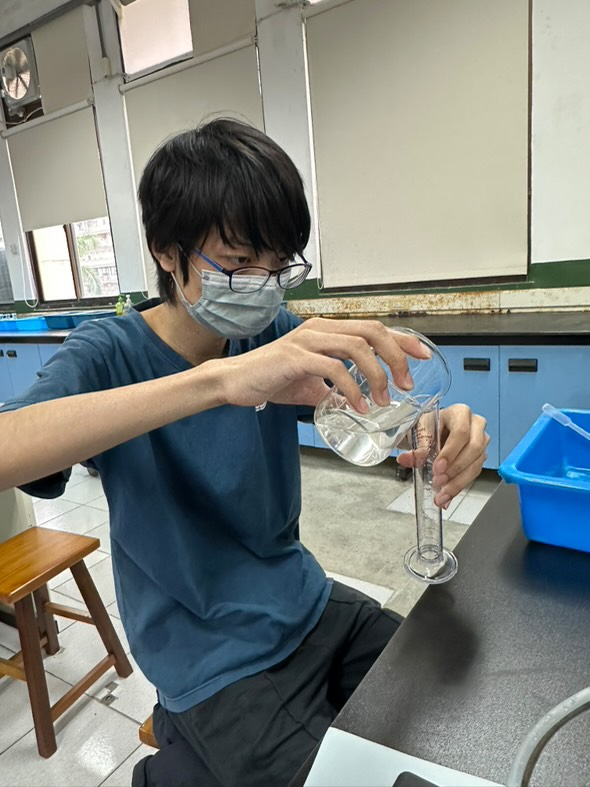
\includegraphics[width=\linewidth]{1.jpg}
% \tcblower
%     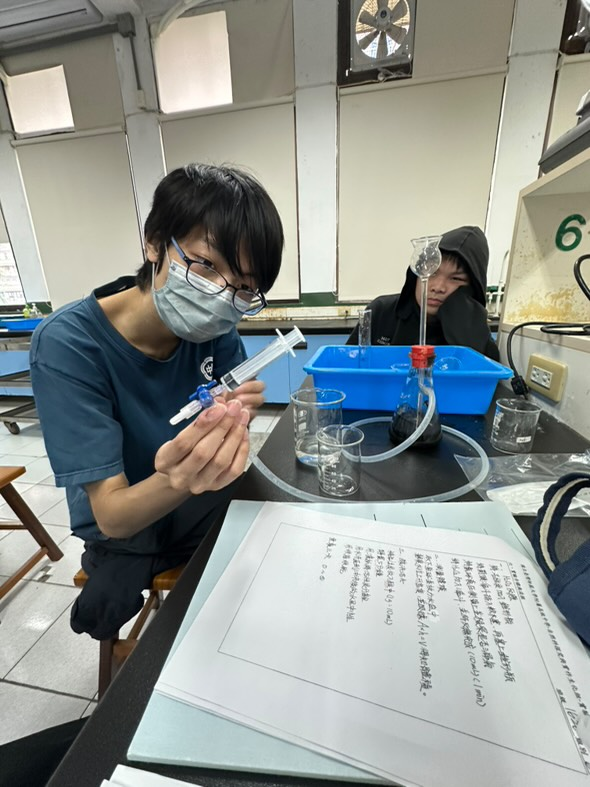
\includegraphics[width=\linewidth]{2.jpg}
% \end{sblock}
%       \begin{sblock}{Violet}
%     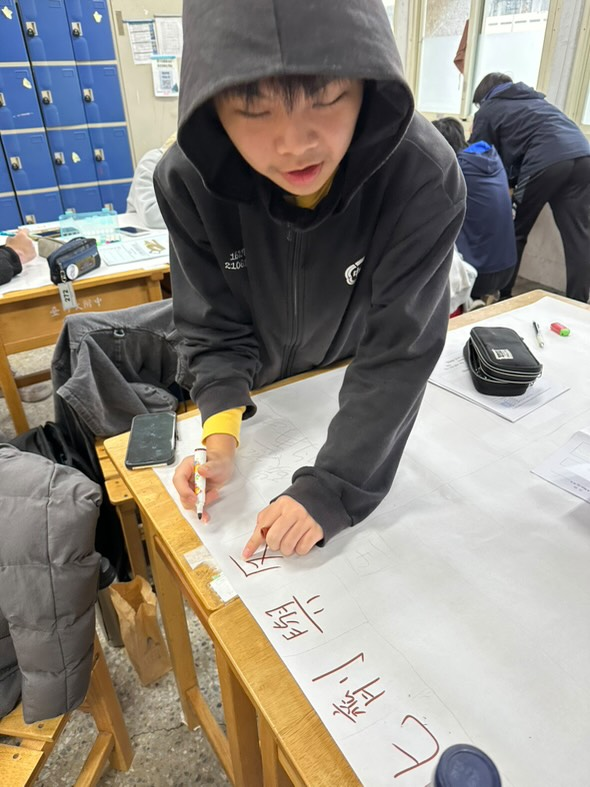
\includegraphics[width=\linewidth]{3.jpg}
% \tcblower
%     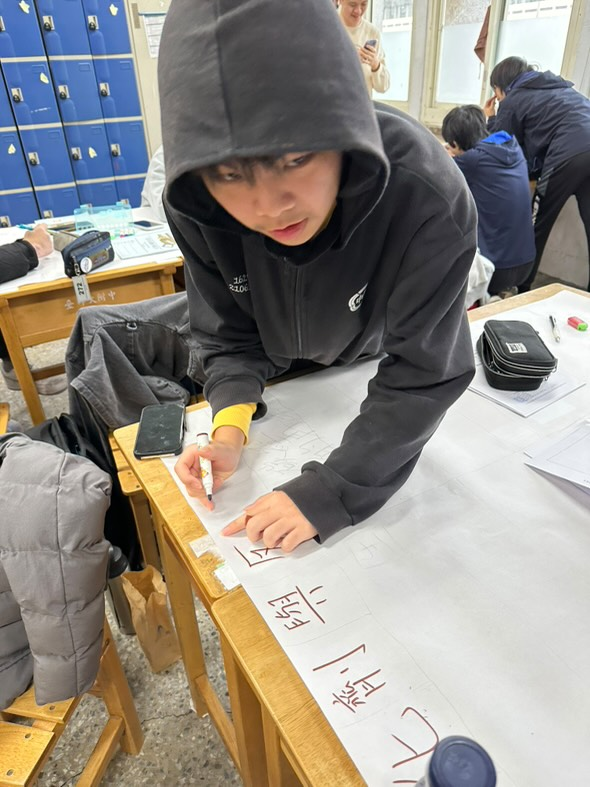
\includegraphics[width=\linewidth]{4.jpg}
% \end{sblock}
% \begin{sblock}{Violet}
% \begin{Huge}
%           實驗海報
% \end{Huge}
% \tcblower
%     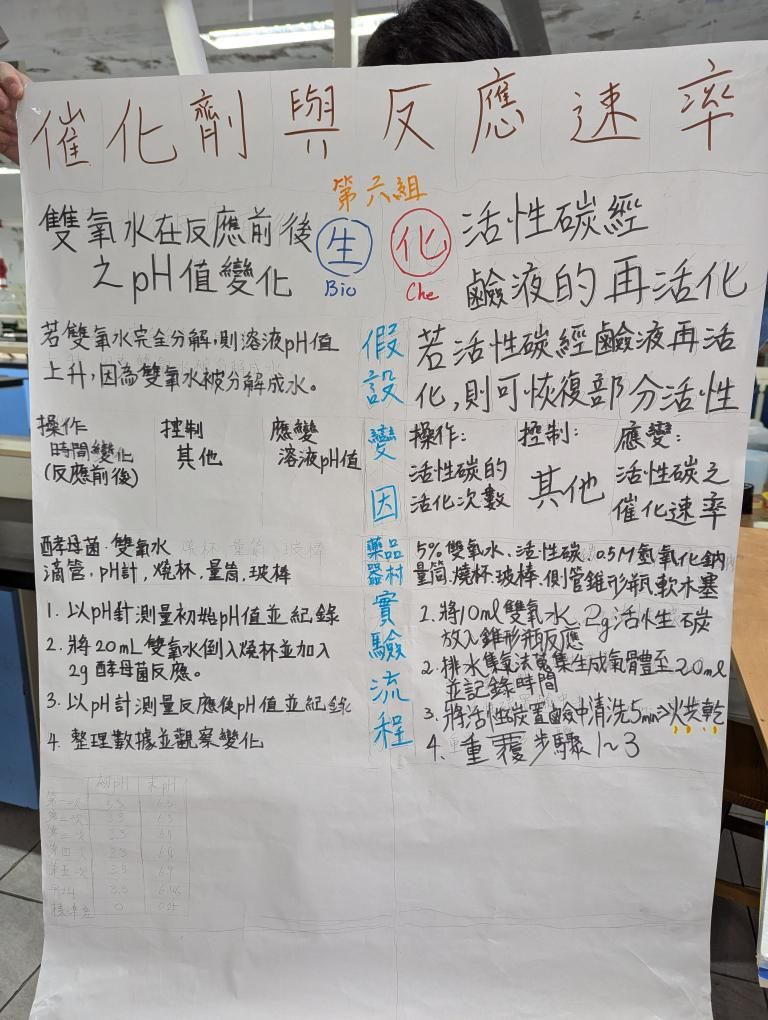
\includegraphics[width=\linewidth]{poster.jpg}
% \end{sblock}
% \end{boxpar}
\begin{boxpar}{Orchid}{學習歷程心得}
    在此次實驗中雖然歷程艱難,測量的實驗數據也不一定準確,但是在過程中也一再體驗與同學在一起合作的重要性。
\end{boxpar}
\end{large}
\end{document}
